\documentclass{standalone}
\usepackage{tikz}
\usetikzlibrary{calc}

\begin{document}

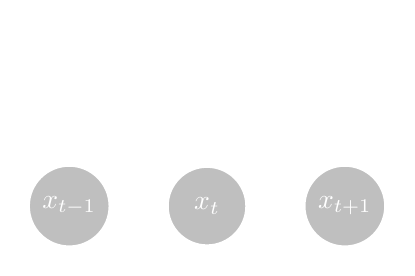
\begin{tikzpicture}[scale=1.5, node distance=1.75cm, every node/.style={circle, draw=white, text=white, minimum size=1cm, thick}, every path/.style={thick, white}]

    % Nodes
    \node[circle, draw=white] (yt1) {$y_{t-1}$};
    \node[circle, draw=white, right of=yt1] (yt) {$y_t$};
    \node[circle, draw=white, right of=yt] (ytp1) {$y_{t+1}$};
    
    \node[circle, draw=white, fill=gray!50, below of=yt1] (xt1) {$x_{t-1}$};
    \node[circle, draw=white, fill=gray!50, below of=yt] (xt) {$x_t$};
    \node[circle, draw=white, fill=gray!50, below of=ytp1] (xtp1) {$x_{t+1}$};
    
    % Edges with filled squares
    \draw (yt1) -- ($(yt1)!0.5!(yt)$) node[rectangle,fill=white,draw=white,minimum size=6pt] {} -- (yt);
    \draw (yt) -- ($(yt)!0.5!(ytp1)$) node[rectangle,fill=white,draw=white,minimum size=6pt] {} -- (ytp1);
    \draw (yt1) -- ($(yt1)!0.5!(xt1)$) node[rectangle,fill=white,draw=white,minimum size=6pt] {} -- (xt1);
    \draw (yt) -- ($(yt)!0.5!(xt)$) node[rectangle,fill=white,draw=white,minimum size=6pt] {} -- (xt);
    \draw (ytp1) -- ($(ytp1)!0.5!(xtp1)$) node[rectangle,fill=white,draw=white,minimum size=6pt] {} -- (xtp1);

\end{tikzpicture}

\end{document}
